%\documentclass[conference]{IEEEtran}
%\documentclass[letterpaper,twocolumn,10pt]{article}
\documentclass{sig-alternate-05-2015}

\usepackage{etoolbox}
\makeatletter
\patchcmd{\maketitle}{\@copyrightspace}{}{}{}
\makeatother

\usepackage{times}
\usepackage{microtype}
\usepackage{thmtools,thm-restate}


\usepackage{mathptmx}
\usepackage[scaled=.90]{helvet}
\usepackage{courier}
\usepackage[override]{cmtt} % make tt font tighter / less ugly

%\usepackage{amsmath,amscd,amssymb,amsthm}
\usepackage[normalem]{ulem}
\DeclareMathAlphabet{\mathcal}{OMS}{cmsy}{m}{n}


%\usepackage[top=1in, bottom=1.25in, left=1.25in, right=1.25in]{geometry}
\usepackage[usenames,dvipsnames]{xcolor}
\usepackage{soul}
\usepackage{colordvi}

\usepackage[yyyymmdd,hhmmss]{datetime}
%\usepackage[clock]{ifsym}
%\usepackage{xcolor}
\usepackage{array}
\usepackage[roman]{sublabel}
\usepackage[override]{cmtt}
\usepackage{cite,color,float}
\usepackage{booktabs}
\usepackage{epsfig,wrapfig,graphics,graphicx}
\usepackage{boxedminipage}
\usepackage{textcomp}
\usepackage{latexsym,fancyhdr}
\usepackage{enumerate}
%\usepackage{algorithm2e,algorithmic}
%\usepackage{algpseudocode}
\usepackage{multirow}
\usepackage{bussproofs}
\usepackage{bbm}
\usepackage{stmaryrd}

\usepackage[framemethod=tikz]{mdframed}
%\usepackage{minted}
\usepackage{listings}

\usepackage{xparse} % argument parsinga -- \edist
\usepackage{xspace}
\allowdisplaybreaks[2]

\setlength{\textfloatsep}{10pt}
\setlength{\floatsep}{0pt}
\setlength{\belowcaptionskip}{0pt}

\newif\iftr\trtrue

\let\labelindent\relax
\usepackage{enumitem}
\newcommand{\unsquish}{
      \setlength{\topsep}{6pt}
      \setlength{\itemsep}{15pt}
      \setlength{\parskip}{6pt}}

\newcommand{\squish}{
      \setlength{\topsep}{0pt}
      \setlength{\itemsep}{0ex}
      \vspace{-1ex}
      \setlength{\parskip}{0pt}}

\setlist{noitemsep,topsep=1pt,parsep=1pt,partopsep=2pt,leftmargin=*}

%\squish

\usepackage{tikz}
\usetikzlibrary{automata,positioning,chains}

\newcommand{\anote}[1]{{\color{magenta}[AM: #1]}}
\newcommand{\tnote}[1]{{\color{green}[TY: #1]}}
\newcommand{\todo}[1]{{\hl{[TODO: #1]}}}

\newcommand{\ignore}[1]{}

%%%%%%%%% Float stuff  %%%%%%%%%%%%%%%%%%%%%%%%%%%%%%%%%%%%%%%
%\renewcommand{\textfraction}{0}
%\renewcommand{\topfraction}{1}
%\renewcommand{\bottomfraction}{1}
%\setcounter{totalnumber}{10}
%\setcounter{topnumber}{10}
%\setcounter{bottomnumber}{10}
%\setcounter{dbltopnumber}{10}
%\renewcommand{\floatpagefraction}{1}
%\renewcommand{\dblfloatpagefraction}{0.8}

%\usepackage{fullpage}
\usepackage{amsmath,amssymb}
%\usepackage{verbatimbox}
\usepackage{boxedminipage}
\usepackage{multirow}
\usepackage{pgfplots}
%\usepackage{subfigure}

%\usepackage{tablefootnote}

%\newtheorem{proposition}{Proposition}
\newtheorem{claim}{Claim}
%\newtheorem{corollary}{Corollary}
\newtheorem{lemma}{Lemma}
%\newtheorem{theorem}{Theorem}

%\setlength{\parskip}{1pt}
%\setlength{\bibsep}{0.0pt}

%\theoremstyle{definition}
\newtheorem{definition}{Definition}
\newtheorem{remark}{Remark}
\newtheorem{theorem}{Theorem}
\newtheorem{fact}{Fact}

\usepackage{algorithm}
\usepackage[noend]{algpseudocode}

\algrenewcommand\textproc[1]{\textsf{#1}}
\algrenewcommand\algorithmicfunction{{}}

\usepackage{hyphenat}
\usepackage{breakurl}
\def\UrlBreaks{\do\/\do-}
%\usepackage[hyphens]{url}
\usepackage{hyperref}
\hyphenation{data-bases}
\hyphenation{un-known}
\hyphenation{asynch-ronous}
\hyphenation{NET-WORK}
\hyphenation{rough-ly}
\hyphenation{crypto-cur-rency}
\hyphenation{pro-ver}
\hyphenation{non-out-source-able}
\hyphenation{con-struct-ed}
\hyphenation{Micro-bench-marks}
\hyphenation{work-er}
\hyphenation{dis-tri-bu-ted}

\newcommand{\name}{AsyncMix\xspace}

\newcommand{\msf}[1]{\ensuremath{{\mathsf {#1}}}}
\renewcommand{\mtt}[1]{\ensuremath{\mathtt {#1}}}
\newcommand{\mcal}[1]{\ensuremath{\mathcal {#1}}}

\newcommand{\poly}{\textnormal{poly}}
\newcommand{\negl}{\textnormal{negl}}

\renewcommand{\P}{\mcal{P}}

\newcommand{\sid}{{\sf sid}}
\newcommand{\sk}{{\sf sk}}
\newcommand{\pk}{{\sf pk}}
\newcommand{\id}{{\sf pk}}
\newcommand{\msg}{{\sf msg}}
\newcommand{\hash}{\ensuremath{{\cal H}}}
\newcommand{\adv}{\ensuremath{{\mathcal A}}\xspace}
\newcommand{\Adv}{\adv}
\newcommand{\A}{\adv}
\newcommand{\samples}{\overset{\$}{\leftarrow}}

\newcommand{\share}[1]{ \ensuremath{{ \llbracket {#1} \rrbracket }} }
\newcommand{\field}{{\ensuremath{\mathbb{F}_p}}}

\begin{document}
\section{Preliminaries}
\label{sec:preliminaries}
\subsection{Polynomial Commitments}
The notion of a polynomial commitment was first formalized by Kate et. al [cite]. In this work, we borrow the PolyCommit interface, but realize the commitment scheme itself with different cryptography. \begin{definition} \label{def:PolyCommit}
A {\em PolyCommit} scheme as defined in [cite] consists of the following algorithms:
\begin{description}
\item [$Setup(1^\kappa, t)$] generates system parameters $SP$ to commit to a polynomial of degree $\le t$. 
  In these system parameters, let $G$ be an algebraic structure for commitments. 
  $Setup$ is run by a trusted or distributed authority. $SP$ can also be standardized for repeated  use.
\item [$Commit(SP,\phi(x))$] outputs a commitment $C$ to a polynomial
  $\phi(x)$ for the system parameters SP, and some associated decommitment information $d$.
    (In some constructions, $d$ can be null.)
\item [$Open(SP,C,\phi(x), d)$] outputs the polynomial $\phi(x)$ used
  while creating the commitment, with decommitment information $d$.  
\item [{$VerifyPoly(SP,C,\phi(x), d)$}] verifies that $C$ is a
  commitment to $\phi(x)$, created with decommitment information $d$. If so, the algorithm outputs $accept$,
  otherwise it outputs $reject$.
\item [$CreateWitness(SP,\phi(x),i,d)$] outputs $\langle i,\phi(i),{w}_i, d_i
  \rangle $, where ${w}_i$ is a witness and $d_i$ is the decommitment information for the
  evaluation $\phi(i)$ of $\phi(x)$ at the index $i$. This algorithm is optional.
  \item [$VerifyEval(SP,C, i,\phi(i), w_i)$] verifies that $\phi(i)$ is
  indeed the evaluation at the index $i$ of the polynomial committed in
  $C$. If so, the algorithm outputs $accept$, otherwise it outputs
  $reject$.
\end{description}
\end{definition} 
Our realization of PolyCommit implements the $Commit$, $CreateWitness$, and $VerifyEval$ functions. We do not use the $Setup$ function of PolyCommit, as the System Parameters in our construction are two generators of a group, which are known to everybody. Hence, we do not require a trusted party or distributed key generation to create $SP$, nor are we constrained in committing only to polynomials of degree $\leq t$.

Unlike Kate et. al's work, we do not use a constant sized commitments, rather we make Pedersen-style commitments to $\phi(x)$ using the coefficients of a "hiding" polynomial $\hat{\phi}(x)$ as detailed in figure ~\ref{polycommit}. This difference does not affect the message complexity of our protocols and the elimination of pairings allows for more efficient computation. Further, by making a Pedersen commitment to the constant of our polynomial, we can utilize efficient Non-interactive Zero Knowledge proofs to alleviate computation down the pipeline. 

\begin{figure}
  \vspace{10pt}
\begin{boxedminipage}{\columnwidth}
  {\centering \textbf{PolyCommit Cryptography} \\}
\begin{itemize}
\item \textbf{Commit}$( \phi(x) ) \rightarrow C,\msf{aux}$:

Sample $deg(\phi(x))$ random numbers as the coefficients for $\hat{\phi}(x)$. With $g$ and $h$ as generators of a group, $C_i = g^{\phi_i}h^{\hat{\phi}_i}, i\in [0,deg(\phi)]$, where $\phi_i$ denotes the $i$'th coefficient of $\phi(x)$. Output the array of $C_i$'s as $C$ and $\hat{\phi}(x)$ as $aux$

\item \textbf{CreateWitness}$(C, aux, i) \rightarrow w_i$:

Interpret $aux$ as $\hat{\phi}(x)$ and solve it at $x=i$. Output $\hat{\phi}(i)$ as $w_i$

\item \textbf{VerifyEval} $(C, i, \phi(i), w_i) \rightarrow bool$:

Assume $C$ is an array of commitments to coefficients of a polynomial and $C_0$ is a commitment to the constant, $C_1$ the coefficient for $x$, and so on.
Return $\prod_{j=0}^{deg(\phi)} {C_j}^{i^j} \overset{?}{=} g^{\phi(i)}h^{\hat{\phi}(i)}$

\end{itemize}
\end{boxedminipage}
\caption{PolyCommit, as used in this paper}
\label{polycommit}
\end{figure}

\subsection{Verifiable Secret Sharing}
\begin{definition} (Secret Sharing)
  A $(t+1)$-secret sharing of a secret $s \in \field$ is a degree-$t$ polynomial $f : \field \rightarrow \field$ such that $f(0) = s$. The shares, one for each of $N$ parties, $\share{s}^{(j)} = f(j)$ are the evaluations of the polynomial at particular points.
\end{definition}

When describing a protocol from the point of view of $P_j$, we omit the superscript in describing the share $\share{s}$.

A verifiable secret sharing scheme for $N$ parties and a dealer $D$ (the dealer may be one of the $N$ parties, but this is not assumed) allows a dealer to create a secret sharing of her input $s$.

\begin{definition}(Asynchronous Verifiable Secret Sharing (AVSS))
  Consider a dealer $D$ and $N > 3t$ parties, where we assume an adversary may corrupt up to $t$ of the parties and possibly the dealer. 
  In an AVSS protocol, the dealer receives input $s \in \field$, and each party $P_i$ may receive an output share $\share{s}^{(i)}$. The protocol must satisfy the following properties:
\end{definition}
\begin{itemize}
\item \emph{(Liveness)}: If the dealer $D$ is honest, then all honest parties output a share \share{s}.
\item \emph{(Secrecy)}: If the dealer $D$ is honest, then the adversary does not learn any information about $s$
\item \emph{(Agreement)}: If any honest party outputs a share $\share{\cdot}$, then there exists a unique value $s$ such that all honest parties output $\share{s}$.
\end{itemize}

Our liveness property implies that as long as the dealer is honest and no more than $t$ nodes are corrupted, then honest nodes are guaranteed output. In Feldman's original verifiable secret sharing protocol, an adversary that corrupts even one node may prevent the protocol from outputting a value.

This agreement property is also written to incorporate the \emph{strong commitment} property due to Backes et al.~\cite{eavss}, in which  agreement the unique value $s$ is already determined  at the time that the first honest party outputs a share (and cannot be influenced thereafter by the adversary).

Backes et al.~\cite{} give a protocol for asynchronous verifiable secret sharing using polynomial commitments. Our solution improves on the performance of this.

\subsection{Communication-optimal reliable roadcast.}
An asynchronous reliable broadcast channel satisfies the following properties:
\begin{itemize}
  \item \emph{(Agreement)} If any two correct nodes deliver $v$ and $v'$, then $v = v'$.
  \item \emph{(Totality)} If any correct node delivers $v$, then all correct nodes deliver $v$
  \item \emph{(Validity)} If the sender is correct and inputs $v$, then all correct nodes deliver $v$
\end{itemize}

While Bracha's~\cite{bra87} classic reliable broadcast protocol requires $O(N^2|v|)$ bits of total communication in order to broadcast a message of size $|v|$, Cachin and Tessaro~\cite{dispersal} observed that erasure coding can reduce this cost to merely $O(N|v| + \lambda N^2 \log N)$, even in the worst case. 
%
%\endnote{Other feasible optimizations on optimistic execution, although for our purposes we focus on the worst-case~\cite{cachin2001secure}.}
%

If the sender is correct, the total running time is three (asynchronous) rounds; and in any case, at most two rounds elapse between when the first correct node outputs a value and the last outputs a value. The reliable broadcast algorithm is shown in Figure~\ref{alg:rbc}.

\begin{figure}[t]
\begin{boxedminipage}{\columnwidth}
{\centering \textbf{Algorithm $\msf{RBC}(D)$ (with Dealer $D$)} \\}
As dealer $D$:
\begin{itemize}
\item upon input$(v)$:
  \begin{itemize}
  \item[] let $\{s_j\}_{j\in[N]}$ be the blocks of an $(N-2f,N)$-erasure coding scheme applied to $v$
  \item[] let $h$ be a Merkle tree root computed over $\{s_j\}$
  \item[] send $\mtt{VAL}(h, b_j, s_j)$ to each party $\P_j$, where $b_j$ is the $j^{th}$ Merkle tree branch
  \end{itemize}
\end{itemize}
As party $\P_i$:
\begin{itemize}
\item upon receiving $\mtt{VAL}(h, b_i, s_i)$ from $\P_\msf{Sender}$,
  \begin{itemize}
  \item[] multicast $\mtt{ECHO}(h,b_i,s_i)$
  \end{itemize} 
\item upon receiving $\mtt{ECHO}(h,b_j,s_j)$ from party $\P_j$, 
  \begin{itemize}
  \item[] check that $b_j$ is a valid Merkle branch for root $h$ and leaf $s_j$, and otherwise discard
  \end{itemize}
\item upon receiving valid $\mtt{ECHO}(h,\cdot,\cdot)$ messages from $N-f$ distinct parties,
  \begin{itemize}
  \item interpolate $\{s'_j\}$ from any $N-2f$ leaves received
  \item recompute Merkle root $h'$ and if $h' \neq h$ then abort        \item if $\mtt{READY}(h)$ has not yet been sent, multicast $\mtt{READY}(h)$
  \end{itemize}
\item upon receiving $f+1$ matching $\mtt{READY}(h)$ messages, if $\mtt{READY}$ has not yet been sent, multicast $\mtt{READY}(h)$
\item upon receiving $2f+1$ matching $\mtt{READY}(h)$ messages, wait for $N-2f$ \mtt{ECHO} messages, then decode $v$
\end{itemize}
\end{boxedminipage}
\caption{Reliable broadcast algorithm from Cachin and Tessaro~\cite{dispersal}, which combines Bracha broadcast~\cite{bra87} with erasure codes to improve efficiency.}
\label{alg:rbc}
\end{figure}

\section{Efficient robust secret sharing}
In our mixing protocol, the the client is only involved in the first round of the protocol, where they send their secret-shared input to the servers. Hence the cost to the client is determined by the Asynchronous Verifiable Secret Sharing (AVSS) protocol.

In an AVSS protocol, a Dealer shares a secret among a set of $N$ nodes (typically the dealer is not among the N nodes, the nodes are servers and the dealer is a client). We envision that the client will be on a resource-constrained device (a laptop) \tnote{I don't know that everyone would consider that to be resource-constrained}, and hence will have limited computation and bandwidth ability. Therefore client cost is our primary performance target. Because our goal is to shuffle inputs provided by multiple different clients, we require \emph{robustness}, in the sense that once we start using a shared input it is guaranteed to be available (even if the Dealer sent malformed data).

The use of a strong form of secret sharing is essential to our use case. If even one piece of malformed or unavailable data makes it into our mix, then the output of the mix will be unrecoverable. To prevent this, we must require that if a server begins executing on the secret shares, then the secret can definitely be recovered. To that end, a fault tolerant AVSS scheme is desirable as it can provide this necessary guarantee even when making very weak assumptions about the stability of protocol participants and the network. Specifically, we desire an AVSS scheme which achieves \textbf{Strong Commitment}, which is the property allows for reconstruction to take place so long as any $2t+1$ parties ($t+1$ honest parties) are online. Strong Commitment is not a definitional property of an AVSS scheme, as it is still possible to reconstruct a secret if not every honest party receives a share, but our overall mixing scheme requires every mixing server to have a share of every secret being mixed. \todo{Add an explanation on why we want byzantine fault tolerance and that N=3t+1 is optimal for that if not explained earlier}

To achieve Strong Commitment, a VSS protocol must guarantee that every participant receives a unique and valid share of the secret, so long as the secret is reconstructable. Previous work achieves this in an asynchronous setting by dealing a bivariate polynomial $f(x,y)$ (with the secret at $f(0,0)$) where participant $P_i$ receives $f(x,i)$, sends $f(j,i)$ to other parties $P_j$, and receives from other parties points to reconstruct $f(i,0)$ which is used as the secret share. In this way, if a party does not receive a message from the dealer, they receive enough information from the other participants to reconstruct their share. Without doing something differently, a univariate polynomial would be unsuitable to achieve Strong Commitment, since a party that didn't receive a message from the dealer must receive their share from other participants, but without any other participants learning the share.

%One may ask, why not use a weaker form of secret sharing? The strong fault tolerance properties of asynchronous verifiable secret sharing are important. We must require that if a server begins executing on the variable, then it can definitely be recovered.

We contribute a robust AVSS protocol that achieves Strong Commitment which is asymptotically more efficient than previous work, and which reaches a practical operating point (to submit a transaction for mixing to $50$ nodes, the client only needs $~2$ seconds of computation)\tnote{Link to experimental section and describe hardware where this is true}. \tnote{Maybe a justification why 50 servers is something we care about?}
Our protocol achieves the following performance for the client: the Dealer only sends a single round of messages and then can disconnect (just one half round). The total bandwidth cost of the dealer is $O(N+\lambda)$, \tnote{What is lambda here?} whereas in the best alternative the cost is $O(N^2)$.

\paragraph{Overview of hbAVSS}

Our key insight is that we can avoid the problem of leaking the shares of other participants in a univariate setting by first encrypting the shares. In our AVSS, the dealer creates a univariate polynomial and encrypts each share with a different key (which can be derived without prior interaction between the dealer and recipients). Every participant receives and helps disperse the same message, which contains all of the encrypted shares, with each participant being able to decrypt one unique share. At this point the dealer is finished and the receivers decide amongst themselves whether everyone has a valid share. Details about our protocol are given below and the full protocol is presented in Figure~\ref{alg:hbavss}.

%The overall flow is that the dealer sends a single round of messages, one to each server. The shares are broadcast through the network, but encryption keeps them secret for each server. The dealer's message also contains authentication information.
%The challenge is ensuring that if any party outputs information, then there will be enough information to do so. We give more detail on the main steps. The detailed protocol is given in Algorithm~\ref{alg:hbavss}.

\begin{enumerate}
\item The Dealer's Portion
\begin{enumerate}
\item \textbf{Sharing and committing}:


  The secret $s$ is first represented as pointwise polynomial $\phi(x)$, where $\phi(0) = s$ and where each party $P_i$ is supposed to receive one share $\phi(i) = \share{s}^{(i)}$.
  
  We refer to PolyCommit as an interface through which a dealer can commit to a polynomial, the innerworkings of which are detailed in Figure ~\ref{polycommit}. $\textbf{Commit}( \phi(x) )$ outputs a commitment $C$, which needs to be sent to all participants. The \textbf{CreateWitness} function creates a data point $w_i$, which when used along with a share in the function \textbf{VerifyEval} allows a recipient to verify that their share is a part of the polynomial committed to by $C$.
  
\item \textbf{Encryption}:


  In our scheme, the dealer sends the same message to every participant. To ensure the secrecy of shares we rely on hybrid encryption. We assume that every recipient possesses a secret key $SK$ and corresponding public key $PK = g^{SK}$ where $g$ is a public generator used for all public keys. We also assume that there exists a PKI where every server's public key can be found. The dealer creates a one-time keypair, for which the public key will be broadcasted. To encrypt party $P_i$'s share, the dealer $P_d$ looks up the public key $PK_i$ and calculates a symmetric key $K^d_i = PK_i^SK_d$, which can also be calculated by $P_i$, and encrypts the share with $\hash(K^d_i)$. This specific construction is chosen to allow parties to share their symmetric key (and prove that it is correctly calculated) without revealing their secret key.
\item \textbf{Reliable Broadcast}:
  The dealer's only communication consists of a single message, the first message in the ReliableBroadcast subprotocol. This message includes the encrypted shares for all participants, encrypted witnesses for all of the shares, commitments to the coefficients of the polynomial, and a public key that recipients can use to derive their shared key.
%Section~\ref{sec:preliminaries}
As described in Section~\ref{sec:preliminaries}, the message is erasure encoded into subshares, and one subshare is sent to each node. A merkle tree is built over the subshares for authentication and each subshare is sent along with its merkle tree branch. If any the servers receive the message $\{z_i\}$ as output, then all the honest servers are guaranteed to receive output $\{z_i\}$. The dealer's cost in this reliable broadcast is just that of broadcasting $O( N log N )$ bits using the efficient reliable broadcast scheme due to Cachin and Tessaro, as in HoneyBadgerBFT.
\end{enumerate}
\item The Recipients' Portion
\begin{enumerate}
\item \textbf{Share Verification}:
  After the reliable broadcast, each party $P_i$ attempts to decrypt their corresponding share and witness. If decryption is successful and \textbf{VerifyEval} returns \textit{True}, then $P_i$ will relay an \mtt{OK} message.%
\footnote{This additional round can be suppressed by modifying Reliable Broadcast, as we discuss in the Appendix \anote{TODO}, but for simplicity we keep the existing interface).}
  Once enough peers $(2t+1)$ report \mtt{OK}, it is safe to use $\share{s}$ in further calculations.

\item \textbf{Handling a faulty dealer}:

   Handling the case of a faulty dealer is the trickiest part of the protocol. Because we are not using a bivariate polynomial, if $P_i$'s correct share is never sent by the dealer, it can not be recovered without reconstructing $\phi(x)$. We argue that the privacy of a malicious dealer's secret is not worth being concerned about.

The polynomial commitment $C$ is included in the reliable broadcast, so all parties agree on it. The secret shares are directly checked against $C$ prior to outputting any secret share, hence if all honest parties output secret shares $\share{s}$, then $\share{s}$ is guaranteed to be a correct $t$-sharing.

  Since each node waits for reliable broadcast to terminate before proceeding, if any party outputs a share $\share{s}$, then every party $\P_j$ receives the polynomial commitment $C$ as well as every party's encrypted materials. If $P_i$ is dealt a share that either fails to decrypt or fails verification, they send the message (\mtt{implicate}, ${K_d}^i$, $\pi$) to all other participants, where $\pi$ is a Non-Interactive Zero Knowledge Proof that the shared key is correct: $ZK\{(SK_i):g^{SK_i} = PK_i$ and $PK_d^{SK_i} = K_{i,d}\}$. Upon validating that the implicate message is correct, other parties will begin sharing their own shared keys so that $P_i$ can reconstruct $\share{s}^{(i)}$. \tnote{I assume we should we detail this ZK proof somewhere? Appendix perhaps?}
  
%Notice that there are two cases where a secret share can be output, the optimistic path and the pessimistic path. In the optimistic path, an honest party only outputs a share if it receives $2t+1$ \texttt{OK} messages, indicating that at least $t+1$ honest parties have received a correct share, and hence the secret will be able to be recovered through interaction.
  \end{enumerate}
\end{enumerate}

\paragraph{Comparison with eAVSS~\cite{eavss}}
\tnote{Should we compare with other AVSSes too?}
Our protocol, hbAVSS, is closely related to prior AVSS protocols. 
The novelty of hbAVSS is that it uses cryptography to overcome limitations in prior approaches which had an information theoretic flavor. hbAVSS uses a more efficient encrypt-and-broadcast, whereas  prior eAVSS-SC protocol performs an information theoretic secret sharing for each party. Both hbAVSS and eAVSS-SC make use of polynomial commitments, though eAVSS-SC requires the use of pairings, which increase the computational cost.

Both eAVSS-SC and hbAVSS rely on shamir secret sharing, as well as a second layer of ``subshares'' which are propagated through the network for redundancy. However, in order to withstand network failures, we further encode each share as a vector of subshares, and for each share $\share{s}^{(i)}$, we send a subshare $\share{s}^{(i,j)}$ to each other party $P_j$. This provides robustness, since it guarantees that all honest parties can eventually receive their share from the network, even if they cannot communicate with the Dealer.

The two protocols eAVSS-SC and hbAVSS differ in how they represent subshares. The protocols are illustrated in Figure~\ref{fig:avss-illustrate}. The data contained within the dashed lines represents the subshares sent by the Dealer into the network, i.e. the communication complexity at the Dealer.

In eAVSS-SC, the subshares form the columns and rows of a $(t,t)$-degree bivariate polynomial, represented point-valuewise as an $N \times N$ matrix of field elements. One row of this matrix is sent to each party $P_i$, which means it requires $O(N^2)$ network communication to send all the subshares in total. With the bivariate approach, privacy is preserved because each share is Shamir-secret-shared again to create the subshares.

\begin{figure}
  \centering
  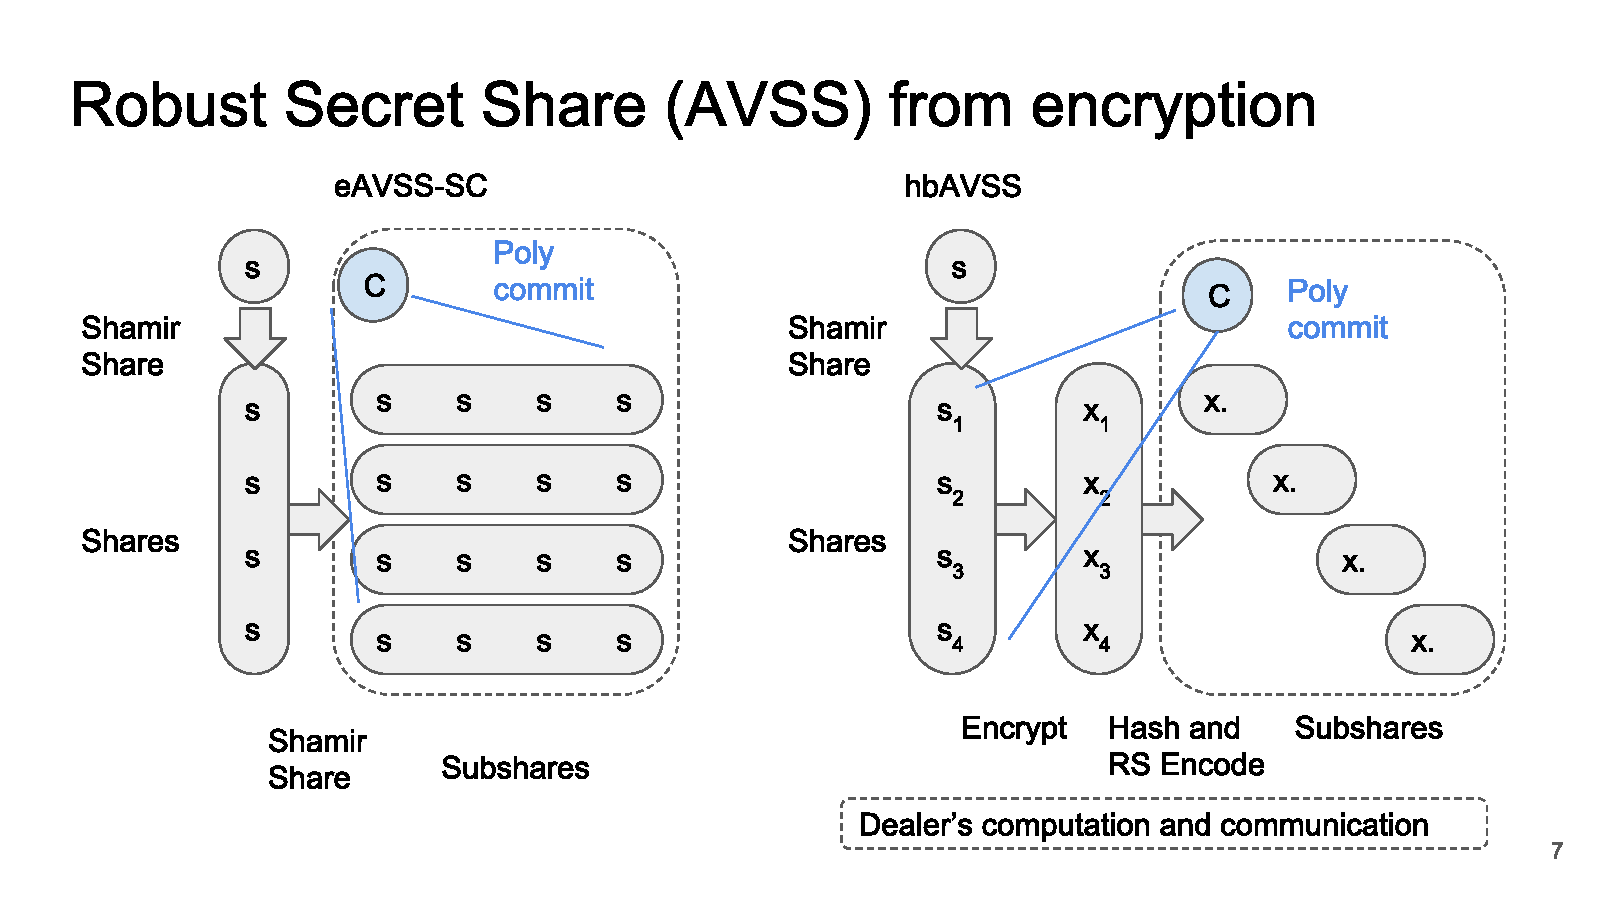
\includegraphics[width=\columnwidth]{graphics/avss-illustration}
  \caption{Illustration of Dealer's communication round in hbAVSS compared with eAVSS-SC}
  \label{fig:avss-illustrate}
\end{figure}

In hbAVSS, we get more efficiency because of using Reed Solomon encoding for the subshares instead of Shamir sharing, resulting in $O(N log N)$ instead of $O(N^2)$ communication cost.
Unlike Shamir, RS encoding does not immediately guarantee privacy. Hence to adapt this for hbAVSS, we restore privacy by applying a public-key encryption step just prior to the RS encoding.
We define hbAVSS in a compositional way, layering on top of an existing reliable broadcast subprotocol ~\cite{dispersal}. The RS Encoding of our subshares is implemented in the Dealer's first message of the Reliable Broadcast subprotocol.

Both eAVSS-SC and hbAVSS use cryptographic Polynomial Commitments and Evaluation Proofs to enable parties to verify the shares they receive. However, in eAVSS-SC evaluation proofs are is used to directly verify each subshare, whereas in hbAVSS the subshares are verified only after decryption. If a party $P_j$ decrypts their subshare $s_j$ and it turns out that polynomial evaluation check fails, then the Dealer is implicated as faulty and the remaining nodes interact to publicly reconstruct the secret.


\begin{figure}
  \vspace{10pt}
\begin{boxedminipage}{\columnwidth}
  {\centering \textbf{Algorithm $\msf{hbAVSS}(D, {\P_i}, s)$ (for party $\P_i$, with dealer $D$)} \\}
  Setup:
\begin{itemize}
\item Each party $P_i$ is associated with a public key $PK_i$, and knows their own secret key $SK_i$ and public generator $g$, such that $PK_i = g^{SK_i}$
\item Setup for the polynomial commitment scheme $SP \leftarrow Setup(1^\lambda)$
\end{itemize}
As dealer $D$:
\begin{itemize}
\item on input $s$:
  \begin{itemize}
  \item Generate random degree-$t$ polynomial $\phi(\cdot)$ with $\phi(0) = s$
  \item Build a polynomial commitment: $C,\msf{aux} \leftarrow \msf{PolyCommit}( \phi )$
  \item Sample an ephemeral secret key \(SK_{d}\) and public key \(PK_{d} = g^{SK_{d}}\)
  \item for each $\P_i$:
    \begin{itemize}
    \item $w_i \leftarrow \msf{CreateWitness}(SP, C, \msf{aux}, i)$
    \item Let a shared symmetric key be $ K_{d,i} = PK_{i}^{SK_{d}} $
    \item $z_i \leftarrow \msf{Enc}_{\hash(K_{d,i})}( \phi(i) \| w_i )$
    \end{itemize}
  \item $\msf{ReliableBroadcast}( C \| PK_d \| \{z_i\}_{i \in [N]} )$
  \end{itemize}
\end{itemize}

As party $\P_i$:
\begin{itemize}
\item wait for output $(C,\{z_j \| PK_{d,i} \})$ from $\msf{ReliableBroadcast}$
  \begin{itemize}
  \item Compute shared key with the dealer \(K_{d,i} = PK_{d,i}^{SK_{i}}\)
  \item $(\share{s}^{(i)} \| w_i) := \msf{Dec}_{\hash(K_{d,i})}(z_i)$
  \item if $\msf{VerifyEval}(SP, C, i, \share{s}^{(i)}, w) = 1$:
    \begin{itemize}
    \item multicast $\mtt{OK}$
    \item wait to receive $\mtt{OK}$ from $2t+1$ different parties
    \item \textbf{output} $\share{s}^{(i)}$
    \end{itemize}
  \item else: Let $\pi_i \leftarrow ZK\{(SK_i):g^{SK_i} = PK_i$ and $PK_d^{SK_i} = K_{i,d}\}$
  \item multicast $(\mtt{IMPLICATE}, {K_{i,d}}, {\pi_i})$
  \end{itemize}

\item on receiving $(\mtt{IMPLICATE}, {K_{j,d}}, {\pi_j})$ from any $\P_j$:
  \begin{itemize}
  \item validate the proof $\pi_j$, counting the message as an \mtt{OK} if validation fails
  \item decrypt share $(\share{s}^{(j)} \| w_j) \leftarrow \msf{Dec}_{\hash(K_{d,j})}(z_j)$
  \item if $\msf{VerifyEval}( SP, C, j, \share{s}^{(j)}, w_j )$ fails:
    \begin{itemize}
      \item multicast $(\mtt{IMPLICATE}, {K_{i,d}}, {\pi_i})$  (only once)
    \end{itemize}
  \item else:
    \begin{itemize}
    \item increment the \mtt{OK} message counter if an \mtt{OK} message has not yet been received from $P_j$
    \item if $t+1$ valid shares have been recovered,  interpolate the polynomial $\phi(\cdot)$ and \textbf{output} $\share{s}^{(i)} = \phi(i)$
    \end{itemize}
  \end{itemize}
\end{itemize}

\end{boxedminipage}
\caption{Our hbAVSS protocol}
\label{alg:hbavss}
\end{figure}


\paragraph{Performance and Security Analysis}

The dealer's communicational cost in this reliable broadcast is $O( N log N )$ bits using the efficient reliable broadcast scheme due to Cachin and Tessaro, as in HoneyBadgerBFT.
\todo{explain the cost more completely}

\textbf{Invariant 1:} If any party outputs $\share{s}$ in optimistic path, then at least $2t+1$ parties have sent \texttt{OK}, and so at least $t+1$ correct parties have received a valid share consistent with $C$.

  With this invariant alone we are not yet done, because it is possible that one party could receive $2t+1$ \texttt{OK} messages and output a value, but some other party may be stuck waiting for \texttt{OK} messages that do not arrive.

  However, because reliable broadcast ensures that each honest party $\P_j$ will eventually receive their encryption $z_j$, we have the following:

\textbf{Invariant 2:} If any party outputs $\share{s}$, then either $2t+1$ honest parties eventually send \texttt{OK}, or else at least one honest party will find that when they decrypt their share, that the share is invalid, and thus broadcast \texttt{IMPLICATE}.

  In case of implication, the idea is that each honest party will broadcast their shares as evidence to implicate the leader. In order to make the evidence non-repudiable, we need to use a non-repudiable encryption scheme. This can be achieved in many ways, the simplest is that we have a committed session key $\sk_i$ and public key $\P_i$ between the dealer and each party $\P_i$, and to implicate a dealer the party $\P_i$ reveals their session key. Once a dealer is implicated, every honest party reveals their share so that the entire secret polynomial can be publicly reconstructed. Notice that this compromises the privacy of the dealer’s secret, but only occurs if the dealer sends invalid data. Since Pi reveals their secret key, if we run different sessions with different dealers, we must ensure that the keys $\sk_i$ and $\P_i$ are isolated between sessions.


\end{document}
